\documentclass[12pt]{article}
% Load packages BEFORE xepersian
\usepackage{geometry}
\usepackage{xcolor}
\usepackage{amsmath}
\usepackage{amsfonts}
\usepackage{graphicx}
\usepackage{pgfplots}
\pgfplotsset{compat=1.18}
\usepackage{booktabs}
\usepackage{longtable}
\usepackage{array}
\usepackage{fancyhdr}
\usepackage{titlesec}
\usepackage{tcolorbox}
\usepackage{hyperref}
% Listings package with custom setup
\usepackage{listings}
% XePersian setup for RTL/LTR support - MUST BE LOADED LAST
\usepackage{xepersian}
\settextfont[Path="./", Extension=".ttf"]{XB-Niloofar}
\setdigitfont[Path="./", Extension=".ttf"]{XB-Niloofar}

% Page setup
\geometry{
	top=2.5cm,
	bottom=2.5cm,
	left=2.5cm,
	right=2.5cm
}
\setlength{\headheight}{16pt} % Adjust headheight to avoid fancyhdr warning

% Colors
\definecolor{codegreen}{rgb}{0,0.6,0}
\definecolor{codegray}{rgb}{0.5,0.5,0.5}
\definecolor{codepurple}{rgb}{0.58,0,0.82}
\definecolor{backcolour}{rgb}{0.95,0.95,0.92}
\definecolor{sectioncolor}{rgb}{0.1,0.4,0.7}
\definecolor{examplecolor}{rgb}{0.9, 0.95, 1.0}
\definecolor{anovacolor}{rgb}{0.95, 0.9, 1.0}

% Header and footer
\pagestyle{fancy}
\fancyhf{}
\fancyhead[R]{\lr{F-Distribution Explained}}
\fancyhead[L]{توضیحات توزیع F}
\fancyfoot[C]{\thepage}

% Section styling
\titleformat{\section}
{\color{sectioncolor}\Large\bfseries}
{\thesection}{1em}{}
\titleformat{\subsection}
{\color{sectioncolor}\large\bfseries}
{\thesubsection}{1em}{}

% Hyperlink setup
\hypersetup{
	colorlinks=true,
	linkcolor=blue,
	filecolor=magenta,      
	urlcolor=cyan,
	pdfpagemode=FullScreen,
	unicode=true,
	pdfencoding=auto
}

\title{
	\begin{center}
		{\Huge \bfseries توزیع F به زبان خیلی ساده} \\
		\vspace{1cm}
		{\large یک راهنمای مفهومی برای مقایسه واریانس‌ها و تحلیل ANOVA}
	\end{center}
}

\author{\href{https://github.com/MohammadMahdi-Sharifbeigy}{محمدمهدی شریف بیگی}}

\date{\today}

\begin{document}
	
	\begin{center}
		\huge\textbf{توزیع F به زبان خیلی ساده}
	\end{center}
	
	\section{ایده حسی}
	
	توزیع F زمانی به کار می‌آید که می‌خواهیم \textbf{نسبت دو واریانس} را با هم مقایسه کنیم. این توزیع برای آزمون‌های فرضیه‌ای استفاده می‌شود که در آن‌ها نیاز داریم بدانیم آیا دو گروه از داده‌ها واریانس (پراکندگی) یکسانی دارند یا خیر.
	
	\textbf{به زبان ساده:} اگر بخواهیم ببینیم که آیا تغییرات درون یک گروه نسبت به گروه دیگر بیشتر است یا نه، از توزیع F استفاده می‌کنیم.
	
	\subsection{شرایط استفاده}
	برای استفاده از توزیع F، شرایط زیر باید برقرار باشد:
	\begin{itemize}
		\item داده‌ها از توزیع نرمال پیروی کنند
		\item نمونه‌ها به‌طور مستقل انتخاب شده باشند
		\item می‌خواهیم نسبت دو واریانس را محاسبه کنیم
		\item تعداد درجات آزادی مشخص باشد
	\end{itemize}
	
	\section{مثال‌های روزمره}
	
	\begin{itemize}
		\item \textbf{مقایسه کیفیت تولید:} آیا ماشین A نسبت به ماشین B محصولات یکنواخت‌تری تولید می‌کند؟
		\item \textbf{مقایسه روش‌های تدریس:} آیا نمرات کلاس A نسبت به کلاس B پراکندگی کمتری دارند؟
		\item \textbf{آزمون ANOVA:} آیا میانگین چندین گروه با هم برابرند؟
		\item \textbf{رگرسیون خطی:} آیا مدل رگرسیون معنادار است؟
		\item \textbf{آزمایش دارو:} آیا اثربخشی یک دارو در گروه‌های مختلف یکسان است؟
	\end{itemize}
	
	\section{پارامترهای اصلی}
	
	توزیع F دو پارامتر دارد:
	\begin{itemize}
		\item $\nu_1$ (نو یک): درجات آزادی صورت - معمولاً مربوط به گروه اول یا بین گروه‌ها
		\item $\nu_2$ (نو دو): درجات آزادی مخرج - معمولاً مربوط به گروه دوم یا درون گروه‌ها
	\end{itemize}
	
	\textbf{مثال:} اگر گروه اول 10 نفر و گروه دوم 15 نفر داشته باشد:
	\begin{align}
		\nu_1 &= 10 - 1 = 9 \\
		\nu_2 &= 15 - 1 = 14
	\end{align}
	
	\section{فرمول چگالی احتمال}
	
	\begin{equation}
		f(x; \nu_1, \nu_2) = \frac{\Gamma\left(\frac{\nu_1 + \nu_2}{2}\right)}{\Gamma\left(\frac{\nu_1}{2}\right) \Gamma\left(\frac{\nu_2}{2}\right)} \left(\frac{\nu_1}{\nu_2}\right)^{\frac{\nu_1}{2}} \frac{x^{\frac{\nu_1}{2} - 1}}{\left(1 + \frac{\nu_1}{\nu_2}x\right)^{\frac{\nu_1 + \nu_2}{2}}}
	\end{equation}
	
	که در آن $x \geq 0$ و $\Gamma$ تابع گاما است.
	
	\section{خصوصیات مهم}
	
	\subsection{میانگین}
	\begin{equation}
		E[X] = \frac{\nu_2}{\nu_2 - 2} \quad \text{برای } \nu_2 > 2
	\end{equation}
	
	\subsection{واریانس}
	\begin{equation}
		\text{Var}(X) = \frac{2\nu_2^2(\nu_1 + \nu_2 - 2)}{\nu_1(\nu_2 - 2)^2(\nu_2 - 4)} \quad \text{برای } \nu_2 > 4
	\end{equation}
	
	\subsection{رابطه با دیگر توزیع‌ها}
	\begin{itemize}
		\item اگر $\nu_1 = 1$، توزیع F به توزیع $t^2$ تبدیل می‌شود
		\item اگر $\nu_2 \to \infty$، توزیع F به توزیع $\chi^2$ نزدیک می‌شود
		\item $F_{1-\alpha}(\nu_1, \nu_2) = \frac{1}{F_\alpha(\nu_2, \nu_1)}$
	\end{itemize}
	
	\section{نمودارهای توزیع F}
	
	
	\begin{figure}[h!]
		\centering
		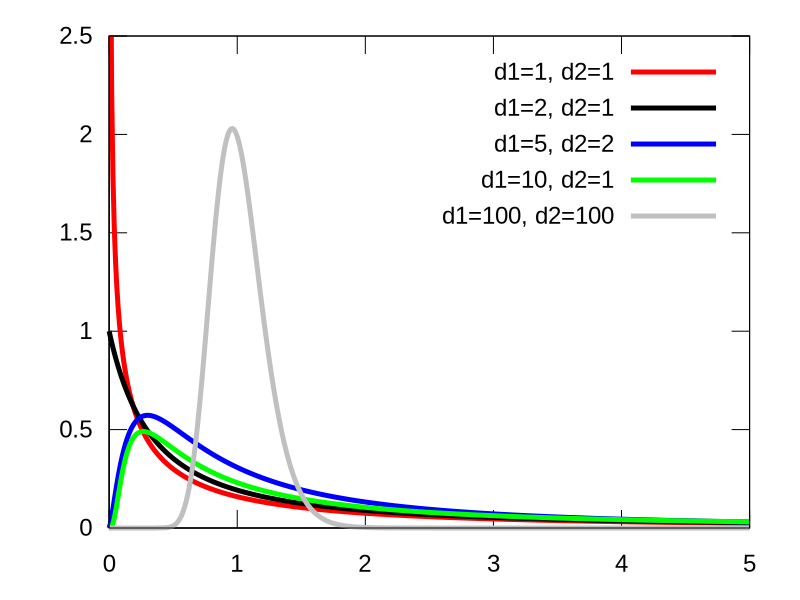
\includegraphics[width=0.9\textwidth]{F_distributions.png}
		\caption{توزیع F با درجات آزادی مختلف. با افزایش درجات آزادی، نمودار به سمت توزیع نرمال میل می‌کند.}
		\label{fig:f_dists}
	\end{figure}
	
	\section{مقایسه با توزیع‌های دیگر}
	
	\begin{center}
		\begin{tikzpicture}
			\begin{axis}[
				width=14cm,
				height=8cm,
				xlabel={$x$},
				ylabel={چگالی احتمال},
				title={مقایسه توزیع F با توزیع‌های مرتبط},
				legend pos=north east,
				grid=major,
				xmin=0, xmax=4,
				ymin=0, ymax=0.8,
				samples=200,
				smooth
				]
				
				% F(5,30) - simplified approximation without gamma function
				\addplot[thick, red] {
					2.5 * x^1.5 / ((1 + 0.167*x)^4)
				};
				\addlegendentry{$F(5,30)$}
				
				% Chi-squared approximation (scaled) - without gamma function
				\addplot[thick, blue, dashed] {
					0.2 * (x^1.5) * exp(-x/2) / 5.66
				};
				\addlegendentry{$\frac{1}{5}\chi^2(5)$ (تقریب)}
				
				% Normal approximation - without sqrt(pi)
				\addplot[thick, green, dotted] {
					exp(-(x-1)^2/0.5) / 1.77
				};
				\addlegendentry{تقریب نرمال}
				
			\end{axis}
		\end{tikzpicture}
	\end{center}
	
	\section{کی از توزیع F استفاده کنیم؟}
	
	\subsection{سوالات کلیدی:}
	\begin{itemize}
		\item آیا می‌خواهم دو واریانس را مقایسه کنم؟ (بله -> \lr{F-test})
		\item آیا داده‌هام از توزیع نرمال پیروی می‌کنند؟ (بله <- شرط لازم)
		\item آیا نمونه‌هام مستقل هستند؟ (بله <- شرط لازم)
		\item آیا می‌خواهم معناداری مدل رگرسیون را آزمون کنم؟ (بله -> \lr{ANOVA})
		\item آیا می‌خواهم میانگین چند گروه را مقایسه کنم؟ (بله -> \lr{ANOVA})
	\end{itemize}
	
	اگر پاسخ‌ها «بله» است، توزیع F احتمالاً انتخاب درستی است.
	
	
	\section{تحلیل واریانس (ANOVA) - توضیح کامل}
	
	\begin{tcolorbox}[colback=anovacolor,colframe=sectioncolor,title=\textbf{ANOVA چیست؟}]
		\textbf{تحلیل واریانس (\lr{Analysis of Variance})} یا ANOVA روشی آماری است که به ما امکان مقایسه میانگین‌های چندین گروه را به‌طور همزمان می‌دهد. به جای اینکه هر دو گروه را جداگانه مقایسه کنیم، ANOVA تمام گروه‌ها را یکباره بررسی می‌کند.
	\end{tcolorbox}
	
	\subsection{چرا ANOVA؟ - مسئله آزمون‌های متعدد}
	
	فرض کنید 4 گروه داریم و می‌خواهیم ببینیم آیا میانگین‌هایشان متفاوت است. اگر از آزمون t استفاده کنیم:
	\begin{itemize}
		\item مقایسه گروه 1 با گروه 2
		\item مقایسه گروه 1 با گروه 3
		\item مقایسه گروه 1 با گروه 4
		\item مقایسه گروه 2 با گروه 3
		\item مقایسه گروه 2 با گروه 4
		\item مقایسه گروه 3 با گروه 4
	\end{itemize}
	
	\textbf{مجموعاً 6 آزمون!} هرچه آزمون بیشتر انجام دهیم، احتمال خطای نوع اول افزایش می‌یابد.
	
	\textbf{ANOVA این مشکل را حل می‌کند:} با یک آزمون واحد تمام گروه‌ها را مقایسه می‌کند.
	
	\subsection{منطق پشت ANOVA}
	
	ANOVA بر این اصل استوار است که کل تغییرات موجود در داده‌ها را می‌توان به دو بخش تقسیم کرد:
	
	\begin{enumerate}
		\item \textbf{تغییرات بین گروه‌ها:} ناشی از اختلاف واقعی بین گروه‌ها
		\item \textbf{تغییرات درون گروه‌ها:} ناشی از تصادف و خطای اندازه‌گیری
	\end{enumerate}
	
	\textbf{اگر تغییرات بین گروه‌ها نسبت به تغییرات درون گروه‌ها زیاد باشد، نتیجه می‌گیریم که گروه‌ها واقعاً متفاوتند.}
	
	\subsection{فرضیه‌های ANOVA}
	
	\textbf{فرضیه صفر ($H_0$):} تمام میانگین‌های گروه‌ها برابرند
	\begin{equation}
		H_0: \mu_1 = \mu_2 = \mu_3 = \ldots = \mu_k
	\end{equation}
	
	\textbf{فرضیه مقابل ($H_1$):} حداقل یکی از میانگین‌ها متفاوت است
	\begin{equation}
		H_1: \text{حداقل یک } \mu_i \neq \mu_j
	\end{equation}
	
	\subsection{مراحل محاسبه ANOVA}
	
	\subsubsection{مرحله 1: محاسبه مجموع مربعات}
	
	\textbf{مجموع مربعات کل (SST):}
	\begin{equation}
		SST = \sum_{i=1}^{k} \sum_{j=1}^{n_i} (x_{ij} - \bar{x})^2
	\end{equation}
	
	\textbf{مجموع مربعات بین گروه‌ها (SSB):}
	\begin{equation}
		SSB = \sum_{i=1}^{k} n_i (\bar{x_i} - \bar{x})^2
	\end{equation}
	
	\textbf{مجموع مربعات درون گروه‌ها (SSW):}
	\begin{equation}
		SSW = \sum_{i=1}^{k} \sum_{j=1}^{n_i} (x_{ij} - \bar{x_i})^2
	\end{equation}
	
	\textbf{رابطه مهم:} $SST = SSB + SSW$
	
	\subsubsection{مرحله 2: محاسبه درجات آزادی}
	
	\begin{itemize}
		\item درجات آزادی بین گروه‌ها: $df_B = k - 1$
		\item درجات آزادی درون گروه‌ها: $df_W = N - k$
		\item درجات آزادی کل: $df_T = N - 1$
	\end{itemize}
	
	که در آن $k$ تعداد گروه‌ها و $N$ تعداد کل مشاهدات است.
	
	\subsubsection{مرحله 3: محاسبه میانگین مربعات}
	
	\textbf{میانگین مربعات بین گروه‌ها (MSB):}
	\begin{equation}
		MSB = \frac{SSB}{df_B} = \frac{SSB}{k-1}
	\end{equation}
	
	\textbf{میانگین مربعات درون گروه‌ها (MSW):}
	\begin{equation}
		MSW = \frac{SSW}{df_W} = \frac{SSW}{N-k}
	\end{equation}
	
	\subsubsection{مرحله 4: محاسبه آماره F}
	
	\begin{equation}
		F = \frac{MSB}{MSW}
	\end{equation}
	
	\textbf{تفسیر:}
	\begin{itemize}
		\item اگر $F$ بزرگ باشد: تغییرات بین گروه‌ها زیاد است <- گروه‌ها متفاوتند
		\item اگر $F$ کوچک باشد: تغییرات بین گروه‌ها کم است <- گروه‌ها مشابهند
	\end{itemize}
	
	
	\subsection{مثال کامل ANOVA}
	
	\subsubsection{مسئله:}
	یک محقق می‌خواهد تأثیر سه روش مختلف تدریس بر نمرات دانش‌آموزان را بررسی کند.
	
	\textbf{داده‌ها:}
	\begin{itemize}
		\item روش A: 85, 88, 90, 87, 86 (میانگین: 87.2)
		\item روش B: 92, 89, 94, 88, 91 (میانگین: 90.8)
		\item روش C: 78, 82, 80, 79, 81 (میانگین: 80.0)
	\end{itemize}
	
	\subsubsection{حل گام به گام:}
	
	\textbf{گام 1: محاسبه میانگین کل}
	\begin{equation}
		\bar{x} = \frac{87.2 \times 5 + 90.8 \times 5 + 80.0 \times 5}{15} = \frac{1290}{15} = 86
	\end{equation}
	
	\textbf{گام 2: محاسبه مجموع مربعات}
	
	\textit{SSB (بین گروه‌ها):}
	\begin{align}
		SSB &= 5[(87.2-86)^2 + (90.8-86)^2 + (80.0-86)^2] \\
		&= 5[1.44 + 23.04 + 36] \\
		&= 5 \times 60.48 = 302.4
	\end{align}
	
	\textit{SSW (درون گروه‌ها):}
	\begin{align}
		SSW_A &= (85-87.2)^2 + (88-87.2)^2 + \ldots = 14.8 \\
		SSW_B &= (92-90.8)^2 + (89-90.8)^2 + \ldots = 22.8 \\
		SSW_C &= (78-80)^2 + (82-80)^2 + \ldots = 10 \\
		SSW &= 14.8 + 22.8 + 10 = 47.6
	\end{align}
	
	\textbf{گام 3: محاسبه درجات آزادی}
	\begin{align}
		df_B &= 3 - 1 = 2 \\
		df_W &= 15 - 3 = 12
	\end{align}
	
	\textbf{گام 4: محاسبه میانگین مربعات}
	\begin{align}
		MSB &= \frac{302.4}{2} = 151.2 \\
		MSW &= \frac{47.6}{12} = 3.97
	\end{align}
	
	\textbf{گام 5: محاسبه آماره F}
	\begin{equation}
		F = \frac{151.2}{3.97} = 38.08
	\end{equation}
	
	\textbf{گام 6: تصمیم‌گیری}
	با $df_1 = 2$ و $df_2 = 12$ در سطح $\alpha = 0.05$، مقدار بحرانی $F_{0.05}(2,12) = 3.89$ است.
	
	چون $38.08 > 3.89$، فرضیه صفر رد می‌شود و نتیجه می‌گیریم که روش‌های تدریس تأثیر معناداری بر نمرات دارند.
	
	\subsection{جدول ANOVA}
	
	\begin{center}
		\begin{tabular}{|l|c|c|c|c|c|}
			\hline
			\textbf{منبع تغییر} & \textbf{مجموع مربعات} & \textbf{درجات آزادی} & \textbf{میانگین مربعات} & \textbf{F} & \textbf{P-value} \\
			\hline
			بین گروه‌ها & 302.4 & 2 & 151.2 & 38.08 & $< 0.001$ \\
			\hline
			درون گروه‌ها & 47.6 & 12 & 3.97 & - & - \\
			\hline
			کل & 350.0 & 14 & - & - & - \\
			\hline
		\end{tabular}
	\end{center}
	
	\subsection{شرایط استفاده از ANOVA}
	
	برای استفاده صحیح از ANOVA، شرایط زیر باید برقرار باشد:
	
	\begin{enumerate}
		\item \textbf{نرمال بودن:} داده‌های هر گروه از توزیع نرمال پیروی کنند
		\item \textbf{استقلال:} مشاهدات مستقل از یکدیگر باشند
		\item \textbf{همگنی واریانس:} واریانس تمام گروه‌ها یکسان باشد
	\end{enumerate}
	
	\textbf{راه‌های بررسی شرایط:}
	\begin{itemize}
		\item نرمال بودن: آزمون شاپیرو-ویلک یا Q-Q plot
		\item همگنی واریانس: آزمون لون یا بارتلت
		\item استقلال: بررسی طراحی مطالعه
	\end{itemize}
	
	\subsection{انواع ANOVA}
	
	\subsubsection{ANOVA یک‌طرفه (\lr{One-Way ANOVA})}
	\begin{itemize}
		\item یک متغیر مستقل (فاکتور) دارد
		\item مثال: تأثیر نوع دارو بر فشار خون
	\end{itemize}
	
	\subsubsection{ANOVA دوطرفه (\lr{Two-Way ANOVA})}
	\begin{itemize}
		\item دو متغیر مستقل (فاکتور) دارد
		\item می‌تواند اثر متقابل را بررسی کند
		\item مثال: تأثیر نوع دارو و جنسیت بر فشار خون
	\end{itemize}
	
	\subsubsection{ANOVA با اندازه‌گیری مکرر (\lr{Repeated Measures ANOVA})}
	\begin{itemize}
		\item همان افراد در شرایط مختلف اندازه‌گیری می‌شوند
		\item مثال: نمرات یک گروه در زمان‌های مختلف
	\end{itemize}
	
	
	\section{کاربردهای عملی}
	
	\subsection{1. آزمون تساوی واریانس}
	فرض کنید دو گروه داریم:
	\begin{itemize}
		\item گروه A: نمونه‌ای با $n_1$ عضو و واریانس نمونه‌ای $s_1^2$
		\item گروه B: نمونه‌ای با $n_2$ عضو و واریانس نمونه‌ای $s_2^2$
	\end{itemize}
	
	آماره آزمون:
	\begin{equation}
		F = \frac{s_1^2}{s_2^2}
	\end{equation}
	
	\subsection{2. تحلیل واریانس (ANOVA)}
	برای مقایسه میانگین k گروه:
	\begin{equation}
		F = \frac{\text{MSB}}{\text{MSW}} = \frac{\text{واریانس بین گروه‌ها}}{\text{واریانس درون گروه‌ها}}
	\end{equation}
	
	\subsection{3. رگرسیون خطی}
	برای آزمون معناداری مدل:
	\begin{equation}
		F = \frac{\text{MSR}}{\text{MSE}} = \frac{\text{میانگین مربعات رگرسیون}}{\text{میانگین مربعات خطا}}
	\end{equation}
	
	\section{مثال عملی ساده}
	
	\subsection{مسئله:}
	دو معلم ریاضی روش‌های مختلفی برای تدریس استفاده می‌کنند. می‌خواهیم ببینیم آیا واریانس نمرات دانش‌آموزان آن‌ها یکسان است یا خیر.
	
	\subsection{داده‌ها:}
	\begin{itemize}
		\item کلاس A: $n_1 = 21$، $s_1^2 = 45$
		\item کلاس B: $n_2 = 16$، $s_2^2 = 30$
	\end{itemize}
	
	\subsection{حل:}
	درجات آزادی: $\nu_1 = 20$، $\nu_2 = 15$
	
	آماره آزمون:
	\begin{equation}
		F = \frac{s_1^2}{s_2^2} = \frac{45}{30} = 1.5
	\end{equation}
	
	\subsection{تفسیر:}
	با مقایسه این مقدار با جدول توزیع F یا استفاده از نرم‌افزار، می‌توان تشخیص داد که آیا این تفاوت معنادار است یا نه.
	
	\section{کاربردهای پیشرفته ANOVA}
	
	\subsection{آزمون‌های پسین (\lr{Post-Hoc Tests})}
	
	زمانی که ANOVA نشان می‌دهد که حداقل یکی از گروه‌ها متفاوت است، برای تشخیص اینکه کدام گروه‌ها متفاوتند، از آزمون‌های پسین استفاده می‌کنیم:
	
	\subsubsection{آزمون توکی (\lr{Tukey HSD})}
	\begin{itemize}
		\item برای مقایسه تمام جفت‌های ممکن گروه‌ها
		\item کنترل نرخ خطای خانوادگی
		\item فرمول: $HSD = q_{\alpha}(k, df_W) \sqrt{\frac{MSW}{n}}$
	\end{itemize}
	
	\subsubsection{آزمون بونفرونی (Bonferroni)}
	\begin{itemize}
		\item محافظه‌کارانه‌تر از توکی
		\item سطح معناداری را تقسیم بر تعداد مقایسه‌ها می‌کند
		\item $\alpha_{adjusted} = \frac{\alpha}{number\ of\ comparisons}$
	\end{itemize}
	
	\subsubsection{آزمون شفه (Scheffé)}
	\begin{itemize}
		\item برای مقایسه‌های پیچیده‌تر
		\item امکان مقایسه ترکیب‌های خطی از میانگین‌ها
	\end{itemize}
	
	\subsection{ANOVA دوطرفه - توضیح کامل}
	
	\subsubsection{مدل ANOVA دوطرفه:}
	\begin{equation}
		Y_{ijk} = \mu + \alpha_i + \beta_j + (\alpha\beta)_{ij} + \epsilon_{ijk}
	\end{equation}
	
	که در آن:
	\begin{itemize}
		\item $\mu$: میانگین کلی
		\item $\alpha_i$: اثر فاکتور اول (سطح i)
		\item $\beta_j$: اثر فاکتور دوم (سطح j)
		\item $(\alpha\beta)_{ij}$: اثر متقابل دو فاکتور
		\item $\epsilon_{ijk}$: خطای تصادفی
	\end{itemize}
	
	\subsubsection{فرضیه‌های قابل آزمون:}
	\begin{enumerate}
		\item \textbf{اثر اصلی فاکتور A:} $H_0: \alpha_1 = \alpha_2 = \ldots = \alpha_a = 0$
		\item \textbf{اثر اصلی فاکتور B:} $H_0: \beta_1 = \beta_2 = \ldots = \beta_b = 0$
		\item \textbf{اثر متقابل:} $H_0: (\alpha\beta)_{ij} = 0$ برای تمام i,j
	\end{enumerate}
	
	\subsubsection{مثال ANOVA دوطرفه:}
	بررسی تأثیر نوع کود (A، B، C) و مقدار آب (کم، متوسط، زیاد) بر عملکرد گیاه.
	
	\begin{center}
		\begin{tabular}{|c|c|c|c|}
			\hline
			\textbf{کود / آب} & \textbf{کم} & \textbf{متوسط} & \textbf{زیاد} \\
			\hline
			A & 15, 17, 16 & 20, 22, 21 & 18, 19, 17 \\
			\hline
			B & 12, 14, 13 & 25, 27, 26 & 23, 24, 22 \\
			\hline
			C & 18, 20, 19 & 24, 26, 25 & 28, 30, 29 \\
			\hline
		\end{tabular}
	\end{center}
	
	\textbf{نتایج تحلیل:}
	\begin{itemize}
		\item اثر نوع کود: معنادار (p < 0.001)
		\item اثر مقدار آب: معنادار (p < 0.001)
		\item اثر متقابل: معنادار (p < 0.05)
	\end{itemize}
	
	\textbf{تفسیر اثر متقابل:} تأثیر نوع کود بسته به مقدار آب متفاوت است. به عنوان مثال، کود B در آب متوسط بهترین عملکرد را دارد.
	
	\subsection{بررسی مفروضات ANOVA}
	
	\subsubsection{1. آزمون نرمال بودن}
	
	\textbf{آزمون شاپیرو-ویلک:}
	\begin{itemize}
		\item $H_0$: داده‌ها از توزیع نرمال پیروی می‌کنند
		\item اگر p-value > 0.05، فرضیه نرمال بودن پذیرفته می‌شود
	\end{itemize}
	
	\textbf{Q-Q Plot:}
	اگر نقاط روی خط قطری قرار گیرند، توزیع نرمال است.
	
	\subsubsection{2. آزمون همگنی واریانس}
	
	\textbf{آزمون لون (Levene):}
	\begin{equation}
		W = \frac{(N-k)}{(k-1)} \frac{\sum_{i=1}^k n_i (\bar{Z_{i.}} - \bar{Z_{..}})^2}{\sum_{i=1}^k \sum_{j=1}^{n_i} (Z_{ij} - \bar{Z_{i.}})^2}
	\end{equation}
	
	که $Z_{ij} = |Y_{ij} - \tilde{Y_i}|$ (انحراف از میانه)
	
	\textbf{آزمون بارتلت (Bartlett):}
	حساس‌تر به انحراف از نرمال بودن، اما دقیق‌تر زمانی که داده‌ها نرمال باشند.
	
	\subsubsection{3. بررسی استقلال}
	\begin{itemize}
		\item بررسی طراحی تحقیق
		\item آزمون دوربین-واتسون برای خودهمبستگی
		\item بررسی الگوهای باقیمانده‌ها
	\end{itemize}
	
	\section{تحلیل قدرت آزمون (\lr{Power Analysis})}
	
	قدرت آزمون احتمال تشخیص صحیح تفاوت واقعی بین گروه‌ها است.
	
	\subsection{فاکتورهای مؤثر بر قدرت:}
	\begin{enumerate}
		\item \textbf{اندازه اثر:} هرچه تفاوت بین گروه‌ها بیشتر باشد، قدرت بالاتر
		\item \textbf{حجم نمونه:} نمونه بزرگ‌تر = قدرت بیشتر
		\item \textbf{سطح معناداری:} $\alpha$ بیشتر = قدرت بیشتر
		\item \textbf{واریانس خطا:} واریانس کمتر = قدرت بیشتر
	\end{enumerate}
	
	\subsection{محاسبه حجم نمونه:}
	برای ANOVA یک‌طرفه:
	\begin{equation}
		n = \frac{2(z_{\alpha/2} + z_\beta)^2 \sigma^2}{\delta^2}
	\end{equation}
	
	که $\delta$ تفاوت مورد انتظار بین گروه‌ها است.
	
	\section{ANOVA غیرپارامتری}
	
	زمانی که مفروضات ANOVA برقرار نیست، از روش‌های غیرپارامتری استفاده می‌کنیم:
	
	\subsection{آزمون کروسکال-والیس}
	\begin{itemize}
		\item معادل غیرپارامتری ANOVA یک‌طرفه
		\item بر اساس رتبه‌بندی داده‌ها
		\item آماره آزمون: $H = \frac{12}{N(N+1)} \sum_{i=1}^k \frac{R_i^2}{n_i} - 3(N+1)$
	\end{itemize}
	
	\subsection{آزمون فریدمن}
	\begin{itemize}
		\item برای طرح‌های با اندازه‌گیری مکرر
		\item زمانی که مفروضات ANOVA مکرر برقرار نیست
	\end{itemize}
	
	\section{نکات عملی و اشتباهات رایج}
	
	\subsection{اشتباهات رایج:}
	\begin{enumerate}
		\item \textbf{عدم بررسی مفروضات} قبل از اجرای ANOVA
		\item \textbf{انجام آزمون‌های متعدد} بدون تصحیح سطح معناداری
		\item \textbf{تفسیر نادرست} p-value (عدم رد ≠ اثبات برابری)
		\item \textbf{نادیده گرفتن اندازه اثر} و تمرکز صرف بر معناداری
		\item \textbf{استفاده از ANOVA} برای داده‌های غیرنرمال شدیداً کج
	\end{enumerate}
	
	\subsection{توصیه‌های عملی:}
	\begin{enumerate}
		\item همیشه مفروضات را بررسی کنید
		\item اندازه اثر را گزارش دهید (\lr{Cohen's d , eta squared})
		\item در صورت معنادار بودن ANOVA، آزمون پسین انجام دهید
		\item نمودارهای مناسب (\lr{boxplot}، بارنمودار) ارائه دهید
		\item حجم نمونه را از قبل محاسبه کنید
	\end{enumerate}
	
	\section{مثال جامع ANOVA در پژوهش}
	
	\subsection{سناریو پژوهشی:}
	محققی می‌خواهد تأثیر چهار روش مداخله روان‌شناختی (کنترل، شناختی، رفتاری، ترکیبی) بر کاهش اضطراب را بررسی کند.
	
	\subsection{طراحی مطالعه:}
	\begin{itemize}
		\item 80 شرکت‌کننده به‌طور تصادفی به 4 گروه تقسیم شدند (n=20 در هر گروه)
		\item نمرات اضطراب قبل و بعد از مداخله اندازه‌گیری شد
		\item متغیر وابسته: تفاوت نمرات (قبل - بعد)
	\end{itemize}
	
	\subsection{نتایج:}
	\begin{center}
		\begin{tabular}{|l|c|c|c|}
			\hline
			\textbf{گروه} & \textbf{میانگین} & \textbf{انحراف معیار} & \textbf{تعداد} \\
			\hline
			کنترل & 2.1 & 3.2 & 20 \\
			\hline
			شناختی & 8.5 & 4.1 & 20 \\
			\hline
			رفتاری & 7.2 & 3.8 & 20 \\
			\hline
			ترکیبی & 12.3 & 4.5 & 20 \\
			\hline
		\end{tabular}
	\end{center}
	
	\textbf{جدول ANOVA:}
	\begin{center}
		\begin{tabular}{|l|c|c|c|c|c|}
			\hline
			\textbf{منبع} & \textbf{SS} & \textbf{df} & \textbf{MS} & \textbf{F} & \textbf{p} \\
			\hline
			بین گروه‌ها & 1285.6 & 3 & 428.5 & 28.97 & < 0.001 \\
			\hline
			درون گروه‌ها & 1123.2 & 76 & 14.8 & - & - \\
			\hline
			کل & 2408.8 & 79 & - & - & - \\
			\hline
		\end{tabular}
	\end{center}
	
	\textbf{آزمون‌های پسین (توکی):}
	\begin{itemize}
		\item کنترل vs شناختی: p < 0.001
		\item کنترل vs رفتاری: p < 0.001
		\item کنترل vs ترکیبی: p < 0.001
		\item شناختی vs رفتاری: p = 0.523 (غیرمعنادار)
		\item شناختی vs ترکیبی: p = 0.019
		\item رفتاری vs ترکیبی: p = 0.002
	\end{itemize}
	
	\subsection{نتیجه‌گیری:}
	تمام روش‌های مداخله نسبت به گروه کنترل مؤثرند. روش ترکیبی بهترین نتایج را دارد و به‌طور معناداری از روش‌های شناختی و رفتاری بهتر است. تفاوت معناداری بین روش‌های شناختی و رفتاری وجود ندارد.
	
	\section{نکات مهم}
	
	\begin{itemize}
		\item توزیع F همیشه مثبت است ($x \geq 0$)
		\item شکل توزیع به درجات آزادی بستگی دارد
		\item با افزایش درجات آزادی، توزیع به نرمال نزدیک می‌شود
		\item نقطه بحرانی توزیع F از جداول آماری یا نرم‌افزار به دست می‌آید
		\item اگر مقدار محاسبه شده از نقطه بحرانی بیشتر باشد، فرضیه صفر رد می‌شود
		\item ANOVA تنها می‌گوید که تفاوت وجود دارد، نه اینکه کدام گروه‌ها متفاوتند
		\item همیشه مفروضات را قبل از تحلیل بررسی کنید
	\end{itemize}
	
	\section{جدول مقادیر بحرانی F}
	
	\begin{center}
		\begin{tabular}{|c|c|c|c|c|c|}
			\hline
			\multirow{2}{*}{$\nu_2$} & \multicolumn{5}{c|}{$\nu_1$} \\
			\cline{2-6}
			& 1 & 2 & 3 & 4 & 5 \\
			\hline
			1 & 161.45 & 199.50 & 215.71 & 224.58 & 230.16 \\
			\hline
			2 & 18.51 & 19.00 & 19.16 & 19.25 & 19.30 \\
			\hline
			3 & 10.13 & 9.55 & 9.28 & 9.12 & 9.01 \\
			\hline
			4 & 7.71 & 6.94 & 6.59 & 6.39 & 6.26 \\
			\hline
			5 & 6.61 & 5.79 & 5.41 & 5.19 & 5.05 \\
			\hline
			10 & 4.96 & 4.10 & 3.71 & 3.48 & 3.33 \\
			\hline
			15 & 4.54 & 3.68 & 3.29 & 3.06 & 2.90 \\
			\hline
			20 & 4.35 & 3.49 & 3.10 & 2.87 & 2.71 \\
			\hline
			30 & 4.17 & 3.32 & 2.92 & 2.69 & 2.53 \\
			\hline
			$\infty$ & 3.84 & 3.00 & 2.60 & 2.37 & 2.21 \\
			\hline
		\end{tabular}
	\end{center}
	
	\textit{مقادیر برای $\alpha = 0.05$}
	
	\section{نتیجه‌گیری}
	
	توزیع F و تحلیل واریانس (ANOVA) ابزارهای قدرتمندی برای مقایسه گروه‌ها و آزمون فرضیه‌های آماری هستند. درک صحیح این مفاهیم برای:
	
	\begin{itemize}
		\item طراحی آزمایش‌های علمی
		\item تحلیل داده‌های پژوهشی
		\item تفسیر نتایج آماری
		\item تصمیم‌گیری مبتنی بر داده
	\end{itemize}
	
	ضروری است. همیشه به یاد داشته باشید که آمار ابزاری است برای کمک به تصمیم‌گیری، نه جایگزین تفکر منطقی و درنظرگیری زمینه مسئله.
	
	\section{منابع}
	
	\subsection{کتب آماری کلاسیک:}
	\begin{itemize}
		\LTR{
		\item Montgomery, D. C. (2017). \textit{Design and Analysis of Experiments}, 9th Edition. John Wiley \& Sons.
		\item Walpole, R. E., Myers, R. H., Myers, S. L., \& Ye, K. (2016). \textit{Probability and Statistics for Engineers and Scientists}, 9th Edition. Pearson.
		\item Field, A. (2018). \textit{Discovering Statistics Using IBM SPSS Statistics}, 5th Edition. SAGE Publications.
		\item Kutner, M. H., Nachtsheim, C. J., Neter, J., \& Li, W. (2005). \textit{Applied Linear Statistical Models}, 5th Edition. McGraw-Hill.
		\item Box, G. E. P., Hunter, J. S., \& Hunter, W. G. (2005). \textit{Statistics for Experimenters: Design, Innovation, and Discovery}, 2nd Edition. John Wiley \& Sons.		
		}
	\end{itemize}
	
	\subsection{مقالات و منابع علمی:}
	\begin{itemize}
		\LTR{
		\item Fisher, R. A. (1925). Statistical Methods for Research Workers. Oliver and Boyd, Edinburgh.
		\item Snedecor, G. W. (1934). Calculation and Interpretation of Analysis of Variance and Covariance. Collegiate Press Inc.
		\item Welch, B. L. (1947). The generalization of Student's problem when several different population variances are involved. \textit{Biometrika}, 34(1-2), 28-35.
		\item Levene, H. (1960). Robust tests for equality of variances. In I. Olkin et al. (Eds.), \textit{Contributions to Probability and Statistics} (pp. 278-292). Stanford University Press.
		\item Tukey, J. W. (1949). Comparing individual means in the analysis of variance. \textit{Biometrics}, 5(2), 99-114.
		}
	\end{itemize}
	
	
\end{document}